\section{Introduction}
\label{sec:intro}

With the popularity of mobile and potable devices, people are getting easier to sketch objects. Sketches have proved to be a powerful and effective tool for communication. A mount of approaches focused on sketch recognition have been studied. But all of them take the recognition accuracy as their only benchmark with ignorance of recognition speed. Mobile and portable devices have more limited computing resources and storage compared to high-performance server or even personal computer. So it is necessary to promote the speed of sketch recognition, but not only accuracy.

Although sketches and images can be visually recognized, they have two main differences: (i) Patterns take more important place in sketch recognition than in image recognition. Sketches vary largely within class. Meanwhile, some sketches coming from different class have similar looking from the high level. But differences can be told from the mid level or low level, e.g., some cats and snowmen are identified easily from their facial part, but hardly from the whole sketches. Objects in images are from the real life. The size of different parts from one object in images are more rationale than that in sketches. (ii) Sketches are sparser than images. Sketches are composed of a group of strokes. For a sketch, most area is blank. Images contains richer information such as texture and dilation. (iii) Sketches have time information. They are generated from a pen. This means a sketch can be viewed as a series of points.

Previous works on sketch recognition are generally borrowed from image classification paradigm. Both conventional sketch recognition and Deep Neural Networks (DNNs) take sketches as images. These methods do not take full advantage of the sparsity of sketches. Besides, in pursuit of high accuracy, they developed different feature fusion methods without the consideration of the model is too bloated to be distributed in mobile devices. Due to special generalization a sketch, it can be represented by only a series of points which takes less storage than represented as an image.

\begin{figure*}
    \center
    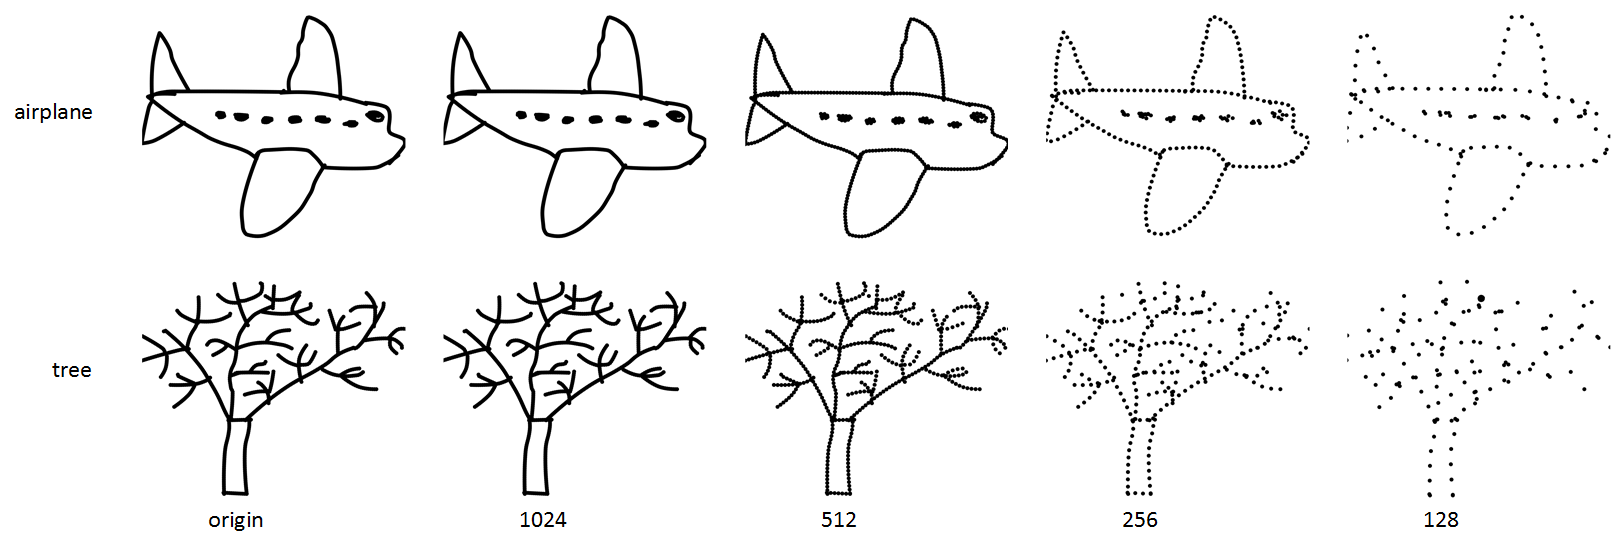
\includegraphics[width=6.5in]{images/resample.png}
    \fcaption{Resample the airplane and the tree into $N$(1024, 512, 256, 128) points.}
    \label{fig:resample}
\end{figure*}

\textbf{Traditional sketch recognition.} In early years, sketch recognition applications \cite{Hse2004SketchedSR, LaViola2004MathPad2AS, Fonseca2000UsingFL} are mainly used for letters and numbers. Hse and Newton \cite{Hse2004SketchedSR} use Zernike moments as features for sketches. Laviola et al. \cite{LaViola2004MathPad2AS} develop an approach for common mathematical symbols recognition. Fonseca and Jorge \cite{Fonseca2000UsingFL} design geometrical features  according to profiles of stokes. These approaches achieve good results because of the simplicity of the symbols.

Symbols from the same class usually have a standard template. Eitz et al. \cite{Eitz2012HowDH} publish a largely free-hand drawn sketches dataset TU-Berlin including common 250 categories of objects. All the objects from same class are drawn by the impression. There are huge difference in class. Eitz et al. extract HOG features of sketches and use a support vector machine(SVM) for classification. Other existing traditional works \cite{LiHSG15, Schneider2014SketchCA} also extract hand-crafted features and use SVMs for classification. The results of traditional approaches are not good on this challenging dataset, for which, humans only acheive 73.1\% recognition accuracy. 

\textbf{DNN-based sketch recognition.} DNN-based approaches have greatly boosted image recognition performance. Sketch-a-Net \cite{Yu2015SketchaNetTB} and DeepSketch \cite{Seddati2015DeepSketchDC} are both proposed deep Convolutional Networks (ConvNets) for sketch recognition. Both of them are derived from image recognition ConvNets. They have larger convolutional kernel size and less convolutional layer compared with general image recognition ConvNets.

Although Sketch-a-Net \cite{Yu2015SketchaNetTB} and DeepSketch \cite{Seddati2015DeepSketchDC} achieve higher recognition accuracy than traditional methods. They still treat each sketch as an image, which do not take full advantages of sparsity of sketches.

\textbf{Point-based 3d model recognition} takes 3d model as group of unordered points. Sketches and 3d models are both a group of points. The difference is: (i)sketches are group of 2d points instead 3d points; (ii) sketch points have time information for they are generated from a pen.

PointNet \cite{qi2017pointnet} summarises the critical points for each class. This ignores the patterns of 3d models. PointNet++ \cite{qi2017pointnetplusplus} uses a hierarchical architecture to summarise patterns of 3d model gradually. Sketches have time information for each points, which shows the way of sketches being generated.

In this paper, we propose a DNN, SketchPointNet, for accelerating sketch recognition and reducing recognition model size, which derived from PointNet \cite{qi2017pointnet}. Comparing with existing DNN-based sketch recognition approaches, we treat each sketch as a series of points which is a sparser representation than image. PointNet++ \cite{qi2017pointnetplusplus} summarize patterns in 3d space, while ours summarize pattern in 2d space. Besides, we incorporate each points of sketches with stroke order information which is unique for sketch points. SketchPointNet is designed with two notable characteristics: (i) a group of micro PointNets are encoded in SketchPointNet hierarchically to capture features of different level; and (ii) micro PointNets summarize patterns along the time series points, while image-based DNN's kernels move in two directions.

Our contributions are summarized as follows: (i)for the first time, we take sketches as a series of points and propose a corresponding DNN to recognize them; (ii) we demonstrate that SketchPointNet has a higher recognition speed and a smaller model size than existing DNN-based approaches.
